\newday{2025-10-18}
    \begin{itemize}
        \item Steps that were used to analyze the spectra of Mrk 501 in XSPEC are given below:
        \begin{enumerate}[I.]
        	\item Reading the data:
        	\begin{verbatim}
XSPEC12> data 1:1 mrk-501_d01_src_I.pha
XSPEC12> data 1:2 mrk-501_d01_src_Q.pha
XSPEC12> data 1:3 mrk-501_d01_src_U.pha
XSPEC12> data 2:4 mrk-501_d02_src_I.pha
XSPEC12> data 2:5 mrk-501_d02_src_Q.pha
XSPEC12> data 2:6 mrk-501_d02_src_U.pha
XSPEC12> data 3:7 mrk-501_d03_src_I.pha
XSPEC12> data 3:8 mrk-501_d03_src_Q.pha
XSPEC12> data 3:9 mrk-501_d03_src_U.pha
        	\end{verbatim}
        	
        	\item Filtering the photons within an energy bandwidth:
        	\begin{verbatim}
XSPEC12> ignore *:**-2.0 8.0-**
        	\end{verbatim}
        	Here the first \verb|*| means to apply this filter on all data groups. Then \verb|**-2.0 8.0-**| means to ignore all photon counts for $E<\num{2}\,\unit{\kilo\eV}$ and $E>\num{8}\,\unit{\kilo\eV}$, i.e. only the the $\num{2}\,\unit{\kilo\eV}\leqslant E\leqslant\num{8}\,\unit{\kilo\eV}$ bandwidth is to be considered.
        	
        	\item Applying the composite model:
        	\begin{verbatim}
XSPEC12> model constant*tbabs*(polconst*powerlaw)
        	\end{verbatim}
        	Here \verb*|constant| models an energy-independent multiplicative factor, \verb|tbabs| models the intervening absorption, \verb|polconst| models a constant polarization at all energies and \verb|powerlaw| models a simple photon power law.
        	
        	\item Parameter \#1 is frozen at 1. Parameters 7 and 13 are untied and thawed. The parameter list prior to fitting looks as follows:
        	\begin{verbatim}
XSPEC12> show par

Parameters defined:
=================================================================
Model constant<1>*TBabs<2>(polconst<3>*powerlaw<4>) Source No.: 1
Active/On
Model Model Component  Parameter  Unit     Value
par  comp
Data group: 1
1    1   constant   factor              1.00000      frozen
2    2   TBabs      nH         10^22    1.00000      +/-  0.0          
3    3   polconst   A                   1.00000      +/-  0.0          
4    3   polconst   psi        deg      45.0000      +/-  0.0          
5    4   powerlaw   PhoIndex            1.00000      +/-  0.0          
6    4   powerlaw   norm                1.00000      +/-  0.0          
Data group: 2
7    1   constant   factor              1.00000      +/-  0.0          
8    2   TBabs      nH         10^22    1.00000      = p2
9    3   polconst   A                   1.00000      = p3
10    3   polconst   psi        deg      45.0000      = p4
11    4   powerlaw   PhoIndex            1.00000      = p5
12    4   powerlaw   norm                1.00000      = p6
Data group: 3
13    1   constant   factor              1.00000      +/-  0.0          
14    2   TBabs      nH         10^22    1.00000      = p2
15    3   polconst   A                   1.00000      = p3
16    3   polconst   psi        deg      45.0000      = p4
17    4   powerlaw   PhoIndex            1.00000      = p5
18    4   powerlaw   norm                1.00000      = p6
_________________________________________________________________
        	\end{verbatim}
        	
        	\item Renormalizing and fitting the model to the spectrum gives the following parameter values:
        	\begin{verbatim}
=================================================================
Model constant<1>*TBabs<2>(polconst<3>*powerlaw<4>) Source No.: 1
Active/On
Model Model Component  Parameter  Unit     Value
par  comp
Data group: 1
1    1   constant   factor           1.00000      frozen
2    2   TBabs      nH        10^22  0.541250     +/-  0.117460     
3    3   polconst   A                7.25453E-02  +/-  1.90183E-02  
4    3   polconst   psi       deg    -49.1296     +/-  7.50921      
5    4   powerlaw   PhoIndex         2.60742      +/-  5.68093E-02  
6    4   powerlaw   norm             9.63365E-02  +/-  8.13714E-03  
Data group: 2
7    1   constant   factor           1.00375      +/-  9.94110E-03  
8    2   TBabs      nH        10^22  0.541250     = p2
9    3   polconst   A                7.25453E-02  = p3
10    3   polconst   psi      deg    -49.1296     = p4
11    4   powerlaw   PhoIndex        2.60742      = p5
12    4   powerlaw   norm            9.62997E-02  = p6
Data group: 3
13    1   constant   factor          0.924722     +/-  1.00195E-02  
14    2   TBabs      nH       10^22  0.541250     = p2
15    3   polconst   A               7.25453E-02  = p3
16    3   polconst   psi      deg    -49.1296     = p4
17    4   powerlaw   PhoIndex        2.60742      = p5
18    4   powerlaw   norm            9.63365E-02  = p6
_________________________________________________________________


Fit statistic: Chi-Squared 131.57 using 149 bins,
								  spectrum 1, group 1.
Chi-Squared      159.05     using 149 bins, spectrum 2, group 1.
Chi-Squared      122.69     using 149 bins, spectrum 3, group 1.
Chi-Squared      130.71     using 149 bins, spectrum 4, group 2.
Chi-Squared      118.58     using 149 bins, spectrum 5, group 2.
Chi-Squared      157.11     using 149 bins, spectrum 6, group 2.
Chi-Squared       60.87     using 149 bins, spectrum 7, group 3.
Chi-Squared       82.38     using 149 bins, spectrum 8, group 3.
Chi-Squared       69.58     using 149 bins, spectrum 9, group 3.
Total fit statistic                 1032.53     with 1334 d.o.f.

Test statistic : Chi-Squared        1032.53     using 1341 bins.
Null hypothesis probability of 1.00e+00 with 1334 degrees of freedom
        	\end{verbatim}
        	
        	\item We are interested in finding the errors in the polarization degree $A$ and polarization angle $\psi$, which are represented by the parameters \verb|A| and \verb|psi| in the \verb|polconst| model component.
        	\begin{itemize}
        		\item To find the 99\% confidence intervals for, say data group 1, we have
        		\begin{verbatim}
XSPEC12> error 6.635 3
XSPEC12> error 6.635 4
        		\end{verbatim}
        		
        		\item To find the 1$\sigma$ confidence intervals for, say data group 1, we have
        		\begin{verbatim}
XSPEC12> error 1.0 3
XSPEC12> error 1.0 4
        		\end{verbatim}
        	\end{itemize}
        	\textbf{Note:} We cannot compute the errors in the same parameters for the other two data groups (i.e. 2 and 3) because these parameters are tied to their counterparts in data group 1. Any attempt to do so will be flagged as an error by XSPEC as follows:
        	\begin{verbatim}
XSPEC12> error 6.635 9
*** Parameter 9 is not a variable model parameter and
	no confidence range will be calculated.
Parameter   Confidence Range (6.635)
XSPEC12> error 6.635 10
*** Parameter 10 is not a variable model parameter and
	no confidence range will be calculated.
Parameter   Confidence Range (6.635)
XSPEC12> error 6.635 15
*** Parameter 15 is not a variable model parameter and
	no confidence range will be calculated.
Parameter   Confidence Range (6.635)
XSPEC12> error 6.635 16
*** Parameter 16 is not a variable model parameter and
	no confidence range will be calculated.
Parameter   Confidence Range (6.635)
        	\end{verbatim}
        	
        	\item To visualize the contour plot, we need the following commands:
        	\begin{verbatim}
XSPEC12> steppar 3 0.00 0.21 50 4 -90 0 60
XSPEC12> plot contour ,,4 1.386, 4.61 9.21 13.81
        	\end{verbatim}
        	The \verb|steppar| command generates a 2D grid of $A$ and $\psi$ values with 50 steps in the range $0<A<0.21$ and 60 steps in the range $-\ang{90}<\psi<\ang{0}$.
        	
        	The \verb|plot contour| command plots contours at 50\% (\verb|1.386|), 90\% (\verb|4.61|), 99\% (\verb|9.21|) and 99.9\% (\verb|13.81|) confidence levels for 2D errors in $\chi^2$.
        \end{enumerate}
        
        \item To estimate the MDP$_{99}$ using PIMMS, we need to do the following:
        \begin{enumerate}
        	\item Determine the model flux in the $\num{2}\,\unit{\kilo\eV}\leqslant E\leqslant\num{8}\,\unit{\kilo\eV}$ bandwidth:
        	\begin{verbatim}
XSPEC12> flux 2.0 8.0
Spectrum Number: 1, 2, 3
Data Group Number: 1
Model Flux  0.015886 photons (8.7966e-11 ergs/cm^2/s) range
	(2.0000 - 8.0000 keV)

Spectrum Number: 4, 5, 6
Data Group Number: 2
Model Flux  0.015945 photons (8.8297e-11 ergs/cm^2/s) range
	(2.0000 - 8.0000 keV)

Spectrum Number: 7, 8, 9
Data Group Number: 3
Model Flux   0.01469 photons (8.1345e-11 ergs/cm^2/s) range
	(2.0000 - 8.0000 keV)
        	\end{verbatim}
        	
        	\item Collect the following values from the best-fit parameters so far:
        	\begin{align*}
        		n_H&=\num{0.540529e22}\,\unit{\per\centi\metre\squared}\qq{(Galactic H column density)} \\
        		\Gamma&=2.60715\qq{(photon index from powerlaw)} \\
        		\expval{F}&=\qty(\dfrac{8.7966+8.8297+8.1345}{3})\num{e-11}=\num{8.5869e-11}\qq{(avg. flux from 3 detectors)}
        	\end{align*}
        	
        	\item Enter these values, along with some more, in \href{https://heasarc.gsfc.nasa.gov/cgi-bin/Tools/w3pimms/w3pimms.pl}{WebPIMMS} as shown:
        	\begin{figure}[h!]
        		\centering
        		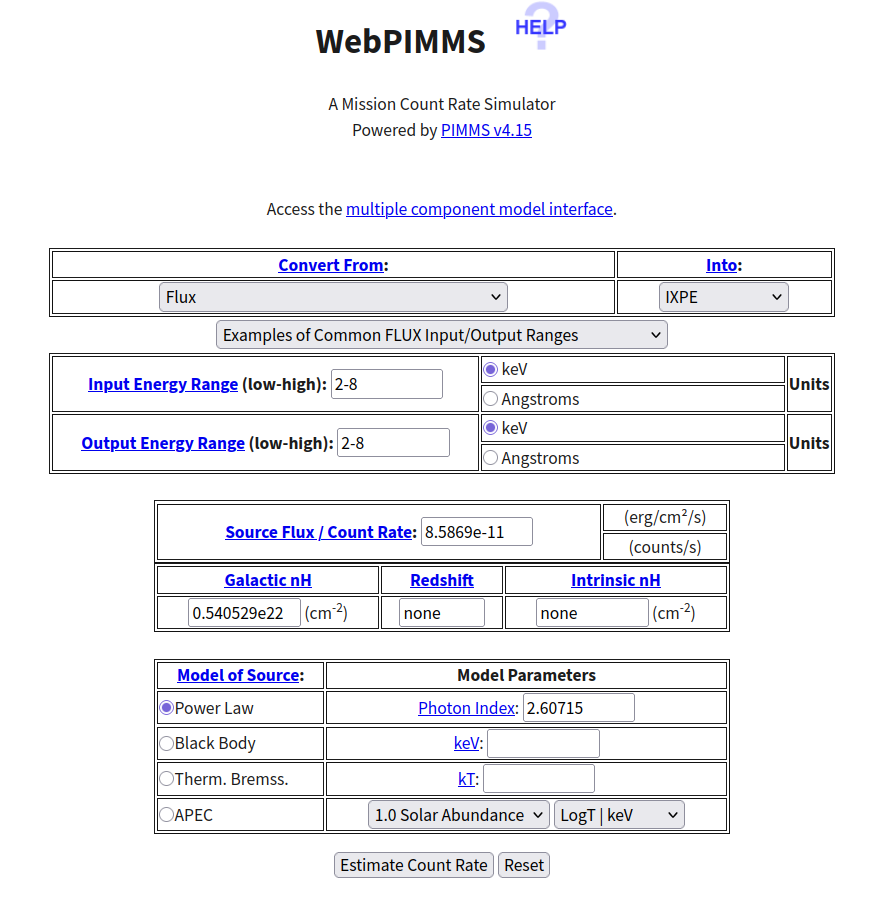
\includegraphics[width=0.8\textwidth]{2025/10/fig_webpimms-input.png}
        	\end{figure}
        	
        	\item \href{https://heasarc.gsfc.nasa.gov/cgi-bin/Tools/w3pimms/w3pimms.pl}{WebPIMMS} computes and displays the predicted count rates and MDP$_{99}$ values using different algorithms, some of which are shown below:
        	\begin{figure}[h!]
        		\centering
        		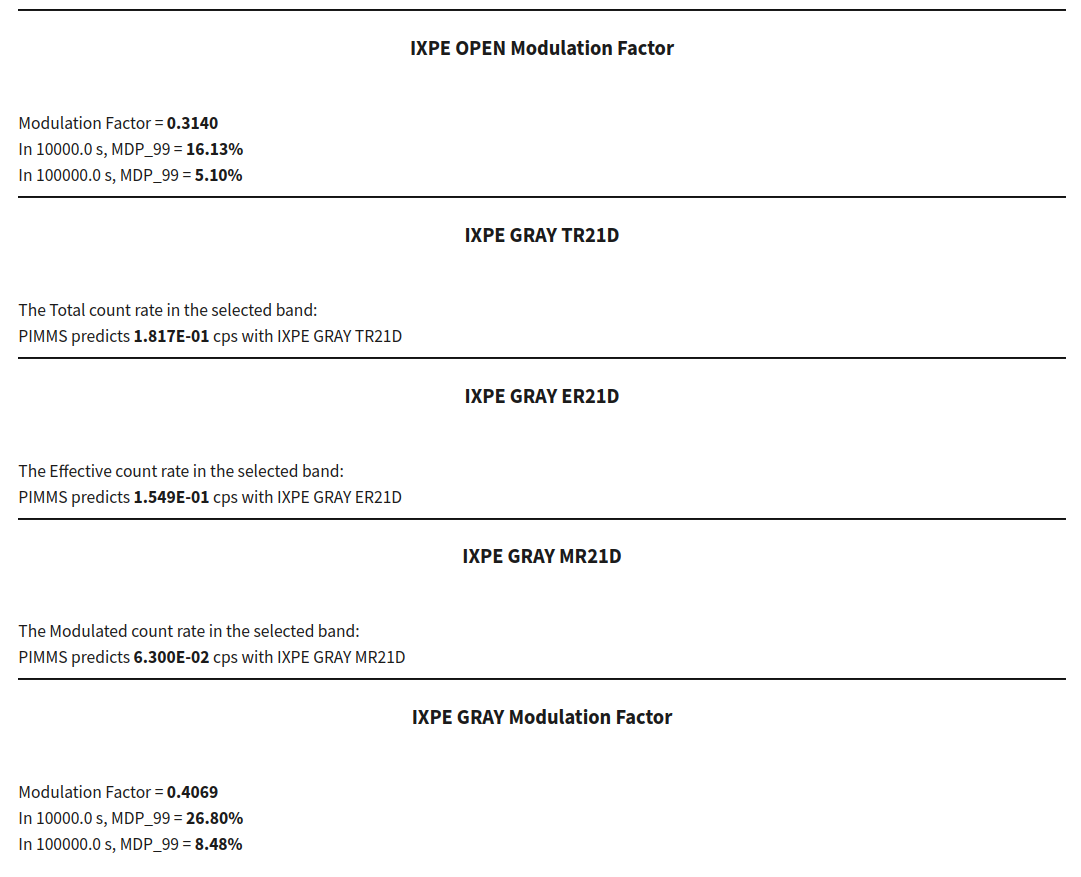
\includegraphics[width=0.9\textwidth]{2025/10/fig_webpimms-output.png}
        	\end{figure}
        	We find, for instance, under `IXPE OPEN Modulation Factor', that for an exposure time of $\num{100}\,\unit{\kilo\second}$, the MDP$_{99}$ is 5.15\%.
        	\begin{align*}
        		T=\num{100}\,\unit{\kilo\second}&\implies\text{MDP}_{99}=5.10\%=0.051
        	\end{align*}
        	
        	Now MDP$_{99}$ scales with exposure time $T$ as $\text{MDP}_{99}\propto\dfrac{1}{\sqrt{T}}$. So we have
        	\begin{align*}
        		\dfrac{\text{MDP}_{99}(\text{actual})}{\text{MDP}_{99}(\text{simulated})}=\sqrt{\dfrac{T(\text{simulated})}{T(\text{actual})}}
        	\end{align*}
        	
        	Running the \verb|show data| command gives us the actual exposure time (e.g. for $I$ spectrum by detector \#1) to be $97800\,\unit{\second}=97\,\unit{\kilo\second}$.
        	
        	Therefore, substituting $T(\text{simulated})=100\,\unit{\kilo\second}$, $T(\text{actual})=97\,\unit{\kilo\second}$ and $\text{MDP}_{99}(\text{simulated})=5.10\%$ above, we obtain
        	\begin{align*}
        		\text{MDP}_{99}(\text{actual})&=\sqrt{\dfrac{100}{97}}\qty(5.10\%)=5.18\%=0.0518
        	\end{align*}
        	This implies that, for an \textit{unpolarized source} with
        	the same physical parameters, an IXPE observation will return a value $A>0.0518$ only 1\% (=100\%-99\%, the 99 is from MDP$_{99}$) of the time.
        \end{enumerate}
        
        \item The chain of logic is as follows:
        \begin{enumerate}
        	\item Scale PIMMS number because the real observation time was a bit shorter, i.e. $\text{MDP}_{99}=5.18\%$.
        	
        	\item $\text{MDP}_{99}$ means ``only 1\% chance a zero-polarisation source would look this big or bigger.''
        	
        	\item Measured value of $7.24\%$ (from best-fit) is above $5.18\%$, and the measurement's uncertainty of $1.9\%$ is small (i.e. $5.18/1.9\approx 3.8$).
        	
        	\item Therefore the measured polarisation is very unlikely to be a random fluke -- it is a highly probable real detection.
        \end{enumerate}
    \end{itemize}